% !TEX root = ../thesis-example.tex
%
\chapter{Implementierung}
\label{sec:impl}

Dieses Kapitel behandelt die Implementierung der RapidMiner-Erweiterung \textit{postagger}. Zuerst wird grob auf den technischen Rahmen seitens RapidMiner eingegangen, dann werden im Abschnitt \ref{sec:impl:aims} Ziele der Implementierung angesprochen. \\
Nach einer Übersicht in Abschnitt \ref{sec:impl:structure} über die Komponenten, die Funktionen aus Kap. \ref{sec:concept} implementieren, werden die Komponenten einzeln im Detail vorgestellt.

\section{RapidMiner}
\label{sec:impl:rm}


Die Datenverarbeitungs-Plattform RapidMiner (kurz \textit{RM}) und ihre Erweiterungen sind in Java geschrieben. RapidMiners zentrale Funktionalität ist es, verschiedene Funktionen (\textit{Operatoren}) in einem Modell hintereinanderzuschalten und mit ihnen Daten zu extrahieren und mit verschiedensten Mitteln zu transformieren oder zu untersuchen.

\paragraph{Operatoren} 
funktionieren entfernter betrachtet wie Funktionen in Programmen: Sie nehmen beliebig viele Eingaben mittels \textit{InputPorts} und \textit{Parametern} entgegen, führen eine Aufgabe aus und haben mindestens eine Ausgabe in Form von \textit{OutputPorts}. Alle Operatoren erben von der Superklasse \textit{Operator}. Eine Erweiterung fügt in der Regel solche Operatoren hinzu.
\paragraph{IO-Objekte}
bzw. IOObjects sind die Datenformate im RM-Modell. Sie werden von der Prozesswurzel sowie von Operatoren ausgegeben und können von Operatoren sowie dem Prozess-Ende entgegengenommen werden. Sie erben von der Klasse \textit{IOObject} und können ebenfalls von Erweiterungen hinzugefügt werden. Operatoren können für ihre Inputs definieren, welche Typ von IOObject sie verlangen. Das Prozessmodell ist nicht lauffähig, wenn diese Spezifikation nicht eingehalten wird.

Eine ausführliche Dokumentation von RM findet sich in \cite{rmdoc} und eine Anleitung zum Erstellen von Erweiterungen bei \cite{rmext}.
 Die implementierte Erweiterung baut auf der Erweiterung \textit{Text Processing} auf, die mit ihren Operatoren und insbesondere dem Übergabeobjekt \textit{Document} (fortan auch einfach als Dokument bezeichnet) viel Arbeit übernimmt. Das Format Document ist prinzipiell nur ein Container für Texte, wobei mit den Operatoren von \textit{Text Processing} bereits viel auf diesem Text gearbeitet werden kann. Zusätzlich sind diese Dokumente bereits in der Lage, Sequenzierungen zu kodieren.
 
 Freundlicherweise wurde von der Firma RapidMiner GmbH eine Arbeitslizenz für dieses Projekt zur Verfügung gestellt.

\section{Ziele}
\label{sec:impl:aims}
Diese Erweiterung soll u.A. vom auftraggebenden Lehrstuhl weiterverwendet und -entwickelt werden können. Das heißt, eine gute Dokumentation und Strukturierung der Komponenten steht im Vordergrund. Da die Erweiterung nicht unbedingt von Programmierern benutzt werden soll, muss außerdem auf eine niedrige Fehleranfälligkeit der Implementierung geachtet werden.
\subsection{Erweiterbarkeit}
Mit Hilfe von Interfaces, Superklassen und statischen Methoden soll gewährleistet sein, dass durch das Hinzufügen von Komponenten nur minimale bis keine Änderungen an anderen nötig sind.
\subsection{Robustheit}
Verwendung von Operatoren außerhalb ihres Funktionsbereiches soll entweder von vornherein unmöglich sein oder leicht verständliche und eindeutige Fehlermeldungen ausgeben. Auch der Vergleich von nicht identischen Ergebnissen soll weitgehend unterstützt werden und Probleme, wie in Kap. \ref{sec:concept:sequence:tok} beschrieben, sollten abgefangen werden.

\section{Übersicht}
\label{sec:impl:structure}

 
\begin{figure}[htb]
	\captionsetup{justification=centering,margin=2cm}
	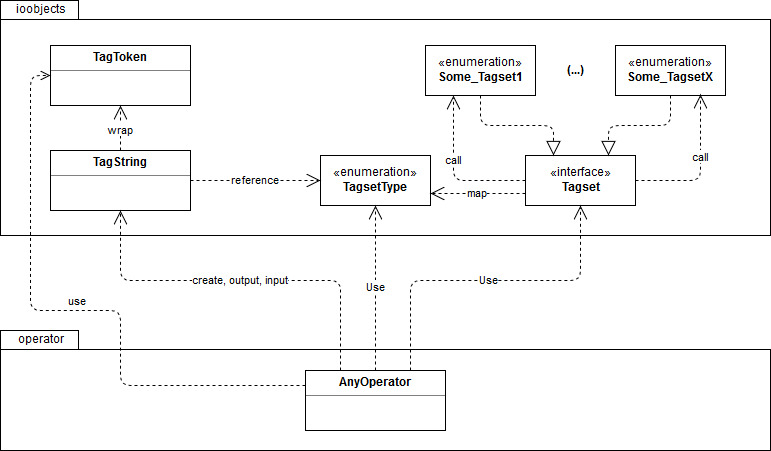
\includegraphics[width=\textwidth]{gfx/uml_rough.jpg}
	\caption{Gekürztes Klassendiagramm der Erweiterung mit Beziehungen}
	\label{fig:impl:structure:overview}
\end{figure}

Abbildung \ref{fig:impl:structure:overview} zeigt einen groben Überblick. Es wurden nur Beispiel-Operatoren und -Tagsets eingezeichnet, sodass nur das Konzept verdeutlicht wird. Es folgt eine kurze Erklärung der verschiedenen Komponenten:

\paragraph{Operatoren} sind Klassen, die von der RapidMiner-Klasse \textit{Operator} erben, und sind auch in der RapidMiner-Nutzeransicht direkt als solche Operatoren vertreten. Alle Operatoren außer dem \textit{Evaluator} beinhalten einen POS-Tagger und wandeln Ein- als auch Ausgangsformate zwischen dem externen RapidMiner-Modell (\textit{Document} oder \textit{TagString} ) und den Vorgaben des Tagging-Algorithmus selbst um. Der Evaluator selbst berechnet die in Kap. \ref{sec:concept} vorgestellten Evaluationsmetriken durch Vergleich von zwei Ergebnissen. Die genaue Funktionsweise des Evaluators wird in Abschnitt \ref{sec:impl:eval} vorgestellt.

\paragraph{Tagsets:} Das Interface Tagset muss von jeder Tag-Enumeration, wie zum Beispiel der des Penn-Treebank-Tagsets implementiert werden. Zusätzlich bietet es statische Methoden, die die Werte der Enumeration TagsetType auf die korrespondierenden Enumerationen abbilden, sowie Abfragen über deren Werte anbieten (hierzu wird der Typ sowie ein Tag verlangt). Auf diese Weise kann ein Tagset mit nur seinem Typen adressiert werden und es ist leicht, das Projekt um ein neues Set zu erweitern.

\paragraph{TagString:} Diese Klasse bietet, wie in Abschnitt \ref{sec:concept:format} angesprochen, ein einheitliches Format für mit Tags versehene Token-Ketten. Sie beschreibt den Tagset-Typen sowie die Zahl an N-Besten Tags pro Token und strukturiert die Tags in Zeilen, die immer dann enden, wenn das letzte Token ein \textit{Separator} ist. 

\section{Tagsets}
\label{sec:impl:tagset}


\begin{figure}[htb]
	\centering
	\captionsetup{justification=centering,margin=2cm}
	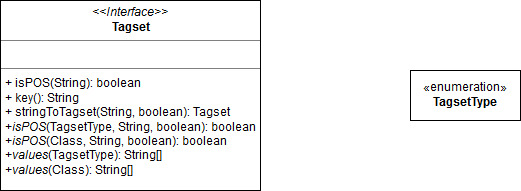
\includegraphics[width=0.7\textwidth]{gfx/tagset_uml.jpg}
	
	\caption{Klassendiagramm-Abschnitt: Tagsets (ohne Beziehungen)} 
	\label{fig:impl:tagset:uml}
\end{figure}

Das Interface \textit{Tagset} realisiert die Aufführung von POS-Tagsets.
Jede Enumeration, die Tagset implementiert, führt eine Gruppe an Tags, wie zum Beispiel die der \textit{Penn Treebank} \cite{Paper:PennBank}, auf und wird von einer Konstante in \textit{TagsetType} repräsentiert. Um eine korrekte Evaluation zu ermöglichen, müssen alle Tags, die auftreten können, in der entsprechenden Enumeration vertreten sein (Der Evaluationsmechanismus zählt nur bekannte Tags als potenziell korrekt). Hat ein Tagger eigene definierte Tags, die vom Standard abweichen, sollten auch diese hinzugefügt werden. Die Enumeration muss folgende Funktionen implementieren:
\begin{description}
\item[key()] liefert den Key des gewählten Tags zurück (falls der Name der Enumerations-Konstante nicht gleich dem Tag ist, würde toString() nicht funktionieren).
\item[isPOS(String key)] liefert genau dann \textsc{true} zurück, wenn ein Tag mit dem übergebenen Key existiert und es ein POS-Tag ist.
\item[stringToTagset(String key, boolean strict)] liefert die Enumerationskonstante für ein Tag mit dem übergebenen Key zurück, sofern es existiert. Falls \textsc{strict} gesetzt ist, wird die Groß- und Kleinschreibung beachtet.
\end{description}

\subsubsection{Mapping von TagsetType auf Tagsets}

Die überladenen statischen Methoden \textit{IsPOS} und \textit{values} haben jeweils eine Variante mit dem Parameter TagsetType, und eine mit dem Parameter Class. Die TagsetType-Variante ersetzt den Tagset-Typen durch seine korrespondierende Enumeration und ruft dann die andere Variante auf. Die andere Variante operiert dann auf dieser Klasse.

Sinn dieser Aufteilung ist es, dass ein Aufruf nicht mit einer Enumeration oder ihrer Implementierung interagieren muss, sondern sie nur via TagsetType adressiert. Wenn eine Änderung an den implementierenden Tagsets vorgenommen wird, muss diese nur im Interface und in TagsetType bekannt werden. Dadurch senkt sich der Aufwand für eine solche Änderung extrem und die Erweiterbarkeit ist für die Menge der Tagsets gewährleistet.

\begin{description}
\item[isPOS(...) (statisch)] gibt die Ergebnisse von der Methode isPOS() der entsprechenden implementierenden Enumeration aus.
\item[values(...) (statisch)] sammelt alle Keys einer implementierenden Enumeration für die isPOS() mit gesetztem \textsc{strict} gilt.
\end{description}

\section{Eingabe und Tokenization}
Zum Einlesen von Text werden bereitgestellte Operatoren von der Erweiterung \textit{Text Processing} (z.B. \textit{read Document}) verwendet. Für diese Aufgabe wurden deshalb keine eigenen Operatoren implementiert. (Satz- und) Wortsequenzierung, wie in \ref{sec:related:pos} definiert, wird ebenfalls von \textit{Text Processing} bereits unterstützt. Hierzu kann ein eingelesenes Dokument einfach mit dem Operator \textit{Tokenize} verarbeitet werden. Eine optimale Sequenzierung liefert der Operator, wenn die Einstellung \textsc{(mode = linguistic tokens)} gesetzt ist.

 Dokumente, die bereits in Tokens zerlegt sind, können mit der Methode \textsc{Document\# getTokenText(): String} abgerufen werden und geben die Token mit Leerzeichen getrennt zurück. Dieses Format ist dann leicht in andere Formate, wie z.B. Listen, zu zerlegen. Um, wie in Abschnitt \ref{sec:concept:sequence} erklärt, Sequenzierungsprobleme zu verhindern, wird Sequenzierung in den Tagging-Operatoren gezielt weggelassen und stattdessen wird ein Davorschalten des Operators \textit{Tokenize} wie oben beschrieben verlangt.

\section{Tag-String als Ergebnisformat}
\label{sec:impl:tagstring}

\begin{figure}[htb]
	\centering
	\captionsetup{justification=centering,margin=2cm}
	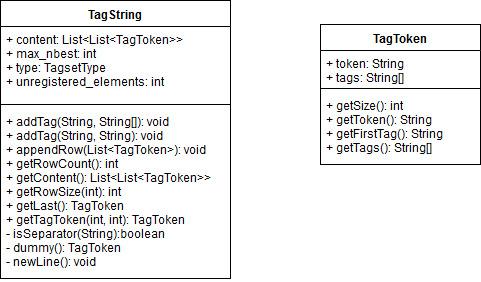
\includegraphics[width=0.7\textwidth]{gfx/tagstring_uml.jpg}
	
	\caption{Klassendiagramm-Abschnitt: TagString (ohne Beziehungen)} 
	\label{fig:impl:tagstring:uml}
\end{figure}

Das in \ref{sec:concept:format} konzeptuell eingeführte Ergebnisformat wird von der Klasse \textit{TagString} realisiert. Solche TagString-Objekte werden vom Parser des Evaluations-Operators (siehe Abschnitt \ref{sec:impl:eval:parsing}) und von Tagging-Operatoren erzeugt und vom Evaluator verwendet. TagStrings sind vorwiegend dazu entworfen, Iteration über Tag-Token-Ketten zu erleichtern und Sequenzierungsfehlern zu entgehen.

\subsection{Metainformationen}
Der TagString bietet die Möglichkeit, beim Erzeugen seinen Tagset-Typen \textsc{[TagsetType type]} festzulegen und zu definieren, wie viele N-Best (Variable \textsc{[int max\_nbest]}) Tags pro Token gespeichert werden sollen. Wird beim Hinzufügen eines Tokens die falsche Menge an Tags hinzugegeben, stellt der TagString von selbst sicher, dass so viele überflüssige Tags entfernt bzw. ungültige Tags hinzugefügt werden, dass die angegebenen \textsc{max\_nbest} Tags vorhanden sind. Der Tagset-Typ wird genutzt, um mittels der statischen Methoden von \textit{Tagset} zu prüfen, ob hinzugefügte Tags (bei mehreren pro Token nur das erste) Teil ihres Tagsets sind. Falls nicht, wird das Tag zwar hinzugefügt, aber der Zähler \textsc{[int unregistered\_elements]} wird inkrementiert.
\subsection{TagToken}
Die TagToken-Objekte sind die Elemente der TagString-Struktur. Sie enthalten ein Token und ein Array an Tags, wobei das erste Tag im Array das First-Best Tag ist. Die Bestandteile können mit den entsprechenden \textsc{get}-Methoden abgefragt werden. Die Methode \textsc{[getSize(): int]} liefert die Größe des Tag-Arrays zurück.

TagTokens wurden eingeführt, um Informationen hinzufügen zu können, ohne Änderungen im restlichen Code zu veranlassen.
\subsection{Aufbau des TagStrings}

Die verschachtelte Liste \textsc{content}, die die TagToken-Objekte sortiert, übernimmt nicht nur die Wort-, sondern auch Satzsequenzierung der Tagging-Ergebnisse. Die innere Liste stellt Sätze dar und wird von der äußeren in Reihenfolge gebracht. 

\subsubsection{Adressierung von Token}
Um das Iterieren über \textsc{content} zu ermöglichen, ohne die Struktur selbst kopieren zu müssen, wurden Hilfsmethoden implementiert. Mit \textsc{getRowCount()} wird die Zahl an Sätzen und mit \textsc{getRowSize(int)} die Zahl an TagToken in einem spezifizierten Satz abgefragt. Mit diesen Informationen kann jedes TagToken via \textsc{getTagToken(int, int)} ausgegeben werden. Ist die Adressierung falsch, wird \textsc{dummy()} aufgerufen, um ein neues TagToken mit ungültigen Tags ("NONE") zurückzugeben. Dadurch sind Iterationen robuster gegen Fehler.

\subsubsection{Serialisierung}
Falls die Zerlegung in Sätze nicht erwünscht ist, kann sie mit der Methode \textsc{serialize()} aufgelöst werden. Dann werden alle inneren Listen zu einer zusammengefasst.

\subsubsection{Hinzufügen von Token}
Beim Hinzufügen von Tagging-Ergebnissen mittels \textsc{addTag(...)} prüft der TagString selbstständig mit Hilfe der Methode \textsc{isSeparator()}, ob das hinzugefügte Token ein Zeilenseparator ist. Als solche Separatoren werden von der Hilfsmethode alle Token identifiziert, die mit Satzzeichen (Punkt, Fragezeichen etc.) beginnen. Ist dies der Fall, wird automatisch die aktuelle Zeile beendet und eine Neue begonnen. 

Den Zeilenumbruch übernimmt der TagString selbst, um eine gleiche Satzsequenzierung verschiedener Ergebnisse zu garantieren, sofern bei diesen die Wortsequenzierung entweder identisch ist oder zumindest jedes Satzzeichen korrekt als eigenes Token abgespalten wurde.

\section{Implementierte Tagging-Operatoren}
Jeder implementierte Tagging-Operator hat folgendes In- und Outputverhalten: Eingelesen wird ein sequenziertes Dokument (es reicht aus, wenn jedes Token durch ein Leerzeichen von Vorgänger und Nachfolger getrennt ist), und ausgegeben dasselbe Dokument, wobei nach jedem Token ein \glqq \ \grqq{} und das Tag folgen. Zusätzlich wird das Tagging-Ergebnis im Format TagString ausgegeben.

\paragraph{NLP4J}
(Dokumentation: \cite{choi}) ist der laut eigenen Angaben leistungsfähigste der implementierten POS-Tagger. Er kann bei der Initialisierung mit trainierten Modellen und Lexika konfiguriert werden. Das eröffnet die Möglichkeit, diese Modelle per Parameter wählbar zu machen, oder sogar via Text-Parameter eigene Modelle und Lexika einzufügen. In dieser Implementierung sind Modell und Lexikon jedoch festgesetzt.
\paragraph{LingPipe}
(Dokumentation: \cite{Lingpipedoc})ist, wie der NLP4J-Algorithmus, mit einem Modell initialisierbar. Die drei verschiedenen vortrainierten Modelle, die der Implementierung beigefügt wurden, sind zu Demonstrationszwecken alle in einem Parameter wählbar gemacht worden. Allerdings liefert nur das Modell, das auf dem \textit{GENIA Korpus} \cite{GENIA} trainiert wurde, POS-Tags zurück, die dem \textit{Penn Treebank} Tagset entsprechen. Da der Evaluations-Testlauf in Kapitel \ref{sec:eval} sich nur auf letzteres Tagset bezieht, sind andere Tagsets noch nicht als entsprechende Enumerationen implementiert.
\paragraph{FastTag}
(Quellcode und Dokumentation: \cite{fasttagdoc})ist ein simpler, nicht auf Trainingsdaten beruhender POS-Tagger. Er wurde implementiert, um einen Vergleich zu den anderen, lernenden POS-Taggern zu bieten.




\section{Evaluations-Operator}
\label{sec:impl:eval}
Der Operator \textit{Evaluator} ist die Zentrale Komponente dieser Erweiterung. Er muss die Formate von Goldstandards sowie Tagging-Ergebnisse annehmen und interpretieren können. Neben dem eigentlichen Evaluieren ist also auch das \textit{Parsen} eingehender Texte eine wichtige Aufgabe des Operators. 

\subsection{Parsing von Ergebnissen}
\label{sec:impl:eval:parsing}
Werden Ergebnisse als Typ Document ausgegeben oder wird ein Goldstandard mit Operatoren aus \textit{Text Processing} eingelesen, liegt ein Document-Objekt mit einem Kodierungsformat vor. Dieses Dokument muss mittels Parsing-Techniken in das TagString-Format transformiert werden, damit eine Evaluation darüber stattfinden kann.

Verschiedene Formate kodieren POS-Tags unterschiedlich. Eine einfache Notation ist die bereits aus der Einleitung bekannte Variante, bei der nach jedem Token ein \glqq \textbackslash \grqq{} und dann das Tag folgt. Andere Notationen kodieren zusätzlich Satzstrukturinformationen, sind also geschachtelt, um z.B. Teilsätze zu markieren. Hier gibt es kein Symbol, das eindeutig ein POS-Tag ankündigt. Um die Parser-Methode des Evaluationsoperators präziser arbeiten können zu lassen, wurde ein Parameter hinzugefügt, in dem man das eingelesene Format und damit den Modus des Parsers nennen kann. Es wurden drei Modi (und damit wählbare Parameter) für den Parser implementiert:

\paragraph{Backslash-Notation:} \cite{Smith} In der oben genannten Notation, in der ausschließlich POS via \glqq \textbackslash \grqq{} markiert werden, ist Parsing einfach. In dieser Notation wird jedes Token mit einem Leerzeichen von seinem Vorgänger und Nachfolger getrennt. Letztlich muss nur noch die Struktur
\[ WORD \mbox{\textbackslash} TAG\]
gefiltert werden.

\paragraph{Parenthesis-Notation bzw. Penn-Treebank-Standard:} \cite{Paper:PennBank} In dieser Notationsvariante wird mittels Klammern die Satzstruktur zerlegt. Wichtig ist, dass Token und Tags immer im Format \textsc{(TAG TOKEN)} bzw. \textsc{(TOKEN TAG)} auftreten. Ferner kann ein Tag also nur auftreten, wenn die Struktur
\[ "(" \: WORD \:\: WORD \: ")" \]
erscheint. Es ist sogar anzunehmen, dass diese Struktur \textit{ausschließlich} Token-Tag-Kombinationen kodiert. Der Parser muss also nur diese Struktur finden und identifizieren, ob eines der beiden Worte ein gültiges POS-Tag ist.

\paragraph{None:} Falls die Notation unbekannt ist, versucht der Parser, den Text an allen sinnvollen Symbolen, insbesondere dem Leerzeichen, zu trennen. Alle Substrings werden dann überprüft, ob sie ein POS-Tag sind. Hier können die Token allerdings nicht identifiziert werden und es handelt sich nur um eine Ausweichs-Option. 

Ein neuer Parsing-Modus kann der Methode einfach hinzugefügt werden. Zusätzlich kann die Option \textit{\glqq Ignore Brackets\grqq{}} gewählt werden, falls Klammern für die Formatierung des einzulesenden Textes verwendet wurden (In der Parenthesis-Notation erübrigt sich das), diese werden dann ignoriert.
\\
Der Tagset-Typ des eingelesenen Dokuments und des ausgegebenen TagStrings muss via Parameter angegeben werden.

\subsection{Iteration über TagStrings}
\label{sec:impl:eval:comparison}

Vergleichsfunktionen müssen nur TagStrings entgegennehmen, da andere Formate vom Parser in solche umgewandelt werden. Aufgrund der automatischen Unterteilung von Token-Ketten in Sätze durch TagStrings kann nicht nur Token- sondern auch Satzweise verglichen werden. Iteriert wird also erst über die Sammlung an Sätzen, dann über deren individuelle Token.

Bei identischer Wort-Sequenzierung der beiden Ergebnisse erübrigen sich Überlegungen über die Robustheit des Vergleichsverfahrens. Hier kann davon ausgegangen werden, dass an gleichen Positionen im TagString auch gleiche Token platziert sind. Bei der Iteration werden also keine Probleme entstehen.

Bestehen allerdings Sequenzierungsunterschiede (siehe Abschnitt \ref{sec:concept:sequence}), kann korrektes Iterieren nicht mehr garantiert werden. Darum wird zuerst überprüft, ob die Satzsequenzierung übereinstimmt. Von einer korrekten Sequenzierung wird ausgegangen, wenn beide zu vergleichenden TagStrings dieselben Satz-Anahlen mit \textsc{countRows()} zurückliefern. Ist dies \textit{nicht} der Fall, muss die Satzsequenzierung aufgelöst werden. Dazu wird bei den TagStrings \textsc{serialize()} aufgerufen (Beschreibung siehe Abschnitt \ref{sec:impl:tagstring}). Danach wird wie zuvor iteriert, wobei beide TagStrings effektiv nur noch einzeilig sind, und Wort-Sequenzierungs-Unterschiede nicht abgefangen werden können. Ist die Satzsequenzierung hingegen korrekt, würden solche Unterschiede beim Iterieren über die Token allerdings nur Probleme innerhalb des Satzes verursachen, da beim nächsten untersuchten Satz die Iteration neu starten kann.

Daraus wird erkennbar, warum bei ungleicher Sequenzierung kein garantiert optimaler Vergleich mehr stattfinden kann. Für korrekte Sequenzierung muss also, wenn möglich, unbedingt schon vorher im Prozess gesorgt werden.

\subsection{Berechnung der Metriken}
\label{sec:impl:eval:calc}

Mittels dem erklärten Iterations-Vorgehen aus dem letzten Abschnitt und den Definitionen aus Abschnitt \ref{sec:concept:eval} kann die Berechnung der Evaluationsmetriken beim Vergleich zweier TagStrings leicht erklärt werden.

\subsubsection{Accuracy}
Per-Tag-Accuracy berechnet sich aus der Zahl der beim Vergleichen der TagStrings identischen Tags geteilt durch die Gesamtzahl der Token (bei ungleicher Satzlänge wird die größere Anzahl an Token zur Gesamtzahl hinzugerechnet). Die Per-Sentence-Accuracy besteht analog aus der Zahl absolut identischer Sätze, geteilt durch deren Gesamtzahl.

\subsubsection{Confusion-Matrix}
Die Confusion-Matrix wird wie folgt gebildet: Zuerst muss eine Liste der auftretenden Tags gebildet werden. Diese wird vom Interface \textit{Tagset} statisch angefragt. Die Matrix hat exakt so viele Zeilen und Spalten wie Tags und deren Index repräsentiert das entsprechende Tag in der Tag-Liste. Die Matrix-Positionen \textsc{matrix[X][Y]} repräsentieren Token, deren Goldstandard-Tag in der Tag-Liste Index X hat, und deren Ergebnis-Tag Index Y hat. Per Definition sind für Tag mit Index X die entsprechenden Werte also wie folgt zu berechnen (\textsc{I} sei hier der maximale Index der Tag-Liste):
\[True\: Positive\:(X)\:=\: matrix[X][X]\]
\[False\: Positive\:(X)\:=\: \Bigg(\sum_{i=0}^I matrix[i][X]\Bigg) - matrix[X][X] \]
\[False\: Negative\:(X)\:=\: \Bigg(\sum_{i=0}^I matrix[X][i]\Bigg) - matrix[X][X] \]
\textit{True Negatives} sind für die berechneten Metriken \textit{Precision, Recall und F-Score} nicht interessant. Precision und Recall sind dementsprechend:

\[Precision(X) \:=\: \frac{matrix[X][X]}{\sum_{i=0}^I matrix[i][X]}\]
\[Recall(X) \:=\: \frac{matrix[X][X]}{\sum_{i=0}^I matrix[X][i]}\]
 
Der F-Score wird wie in Kapitel \ref{sec:concept} definiert als harmonisches Mittel von Precision und Recall berechnet. Die Rechnung $\frac{0}{0}$ wird abgefangen, sodass stattdessen null als Ergebnis ausgegeben wird.

\subsubsection{N-Best Tags}
Wurde beim Parameter \textit{Calculate N-Best Distance} ein Haken gesetzt, werden zwei weitere Metriken berechnet:

\paragraph{N-Accuracy:} Diese Variante der Accuracy wird analog zur Per-Tag-Accuracy berechnet. Allerdings werden alle Tags pro Token im Tagging-Ergebnis mit dem korrekten Tag im Goldstandard verglichen. Findet sich unter allen Tags ein Korrektes, wird wie bei der normalen Per-Tag-Accuracy von einem korrekten Tag ausgegangen. Dieser Wert ist also mindestens so hoch wie die Per-Tag-Accuracy desselben TagStrings.
\paragraph{N-Distanz:} Um genauere Einsicht darauf zu liefern, an welcher Stelle das durchschnittliche korrekte Tag unter den besten n stand, wird die durchschnittliche Distanz eingeführt. Ist das erste Tag korrekt, beträgt die Distanz für dieses Token 1, ist das zweite korrekt, ist sie 2, und so weiter. Wird das  korrekte Tag unter den besten n nicht gefunden, lautet die Distanz n+1. Die N-Distanz für einen ganzen TagString ist dann der Durchschnitt aller Distanzen pro Token.

\subsection{Ausgabe}
\label{sec:impl:eval:out}

Da diese Erweiterung zur Weiterentwicklung konzipiert wurde und in eine größere Bilbiothek übernommen werden wird, wurde die Definition eines Evaluations-Formats absichtlich weggelassen.

Als Ersatz liefert der Evaluationsoperator ein Dokument aus, in dem alle berechneten Ergebnisse (und falls gewünscht auch die Confusion-Matrix) textuell wiedergegeben werden. Zusätzlich gibt ein zweiter Output das Ergebnis des Parsers beim eingelesenen Goldstandard aus, sodass überprüft werden kann, ob der Parsing-Prozess korrekt abgelaufen ist.

\section{Zusammenfassung}
\label{sec:system:conclusion}

Der Evaluationsoperator bietet Einsichten über verschiedene Evaluationsmetriken beim Vergleich zweier Tagging-Ergebnisse, wobei einer davon als Goldstandard betrachtet wird. Sind beide Ergebnisse kein Goldstandard, können die beiden \textit{Accuracy}-Werte als Übereinstimmung der Ergebnisse interpretiert werden. Als Tagging-Algorithmen wurden drei unterschiedlich konfigurierbare POS-Tagger in Operatoren verpackt. Während die Tagger ihre Ergebnisse in Textform ausgeben und der Evaluator diese einlesen können, wurde für eine informationsreichere Übergabe von Daten die Datenstruktur TagString definiert. Zusätzlich wurden die verwendbaren Tagsets als Enumerationen definiert.

Mehrere Methoden wurden angewendet, sodass die Erweiterung leicht um neue Tagsets oder Informationen im TagString vergrößern werden kann. Es wurde auch darauf geachtet, dass der Evaluationsoperator möglichst nicht fehleranfällig ist und im Falle eines Fehlers nützliche Informationen an den Nutzer ausgibt.